\clearpage
\section{Adam Timing, Severity, and Warning Memory}

\subsection{Trajectories, event selection, and targets}
The complete comparison has nine full-objective Adam trajectories: MLP rates $.0001/.0003/.001$ and ResNet/Transformer rates $.0003/.001/.003$, each for 1,024 updates with one initialization per model. Initial tensors agree across rates within a model, moments start at zero, and the native coefficients are $(.9,.999)$ with $\epsilon=10^{-8}$ and no clipping, decay, or schedule. Numerical runtimes differ across some arms; hardware effects are not separately randomized.

A loss excursion starts at a strict increase, fixes the preceding state as its baseline, and tracks the peak until the first return to or below that baseline. An excursion still open at the horizon is right-censored. The overview uses a zero-based vertical range for $\eta\widehat\kappa_t$, leaving 13/17/1 negative MLP/ResNet/Transformer values outside view without changing them. Overview shading uses baseline-to-peak intervals whose maximum exceeds baseline by more than 10\%; outlined intervals retain unobserved recovery. These event definitions are distinct from the individual-step targets used below. A sequence of upward updates is not a sequence of independent spikes.

Decisions at $t=1,\ldots,1023$ use only available raw-gradient information. At future offset $h$, the individual target is
\begin{equation}
 Y_{t,h}(\delta)=\mathbf1\{(L_{t+h}-L_{t+h-1})/L_{t+h-1}\geq\delta\},
\end{equation}
with strict positivity for the zero-threshold case. Net targets instead compare $L_{t+h}$ with $L_t$; within-horizon targets compare $\max_{1\leq j\leq h}L_{t+j}$ with $L_t$. The common cohort $t=1,\ldots,1008$ supports all $h=1,\ldots,16$ without changing endpoint composition. A second analysis restricts decisions to $L_t\leq L_{t-1}$; it excludes an already-rising step, not necessarily an ongoing excursion.

Coverage is $\mathrm{TP}/(\mathrm{TP}+\mathrm{FN})$, precision is $\mathrm{TP}/(\mathrm{TP}+\mathrm{FP})$, and the false-positive rate is $\mathrm{FP}/(\mathrm{FP}+\mathrm{TN})$. Precision lift uses the unconditional target frequency in the identical cohort. Undefined ratios remain missing. The flags $D=(\rho_t<0)$, $G=(r_t>1)$, $D\wedge G$, and $\eta\widehat\kappa_t\geq2$ are evaluated before the outgoing update. The angle/norm form of $\eta\widehat\kappa_t>2$ is algebraically equivalent, not a fifth signal.

\begin{table}[H]
\centering\small
\caption{Complete next-step sign accounting in the three displayed high-rate arms. Each signal cell gives flagged increases/flagged decreases; target totals are in the second and third columns. The upper block concerns strictly positive or negative individual changes. The lower block gives confusion counts for the main 0.1\% next-step target, using the same 1,023 decisions; non-target steps include smaller rises. Neither target counts recovered excursions.}
\begin{tabular}{@{}lrrrrrr@{}}
\toprule
Case & Increases & Decreases & $D$ up/down & $G$ up/down & Both up/down & $\eta\widehat\kappa\geq2$ up/down \\
\midrule
MLP & 454 & 569 & 404/412 & 261/285 & 239/218 & 172/136 \\
ResNet & 95 & 928 & 86/214 & 47/277 & 46/116 & 21/15 \\
Transformer & 152 & 871 & 145/376 & 99/322 & 98/203 & 81/66 \\
\bottomrule
\end{tabular}
\medskip
\begin{tabular}{@{}lrrr@{}}
\toprule
0.1\% target: TP / FP / FN / TN & MLP & ResNet & Transformer \\
\midrule
$L_t>L_{t-1}$ & 236/219/210/358 & 35/60/53/875 & 78/74/64/807 \\
$\rho_t<0$ & 398/418/48/159 & 81/219/7/716 & 135/386/7/495 \\
$\|g_t\|>\|g_{t-1}\|$ & 258/288/188/289 & 46/278/42/657 & 93/328/49/553 \\
$\eta\widehat\kappa_t\geq2$ & 172/136/274/441 & 21/15/67/920 & 79/68/63/813 \\
\bottomrule
\end{tabular}
\end{table}

For the main 0.1\% target, the event totals are 446/88/142. Classification accuracy is $(\mathrm{TP}+\mathrm{TN})/1023$. Warning hit rate is precision, and its lift uses the event frequency above. The naive history rule flags any strictly positive preceding change; it does not inspect the next loss. Strict angle/norm and non-strict projected-response thresholds agree here because no measured value equals two. The table exposes the false alarms and misses behind the main comparison.

Warning memory flags a decision if a condition occurred at any of the last $w$ states, including the current one. All $w=1,\ldots,16$ use $t=16,\ldots,1023$, and each target update is counted once. Enlarging the memory window enlarges the flag set; improved coverage must be assessed with its additional false alarms. Similarly, a longer future search window increases the opportunity for a positive target.

These grids are exploratory characterization on previously inspected trajectories. Thresholds, horizons, and selected high-rate displays do not constitute prospective confirmation. Temporal dependence and one initialization per model preclude independent-seed confidence intervals. A validated predictor would require fixed targets and horizons, temporal separation, loss-history and norm baselines, and fresh-seed evaluation.

Across all nine rates, 9,207 eligible decisions contain 2,233 increases and 6,974 decreases. The $\eta\widehat\kappa_t\geq2$ condition covers 853 increases and flags 955 decreases. On the common 1,008-state high-rate cohort, Transformer coverage of individual increases of at least 10\% is 22/26, 25/26, and 26/26 at offsets one, two, and three. At offset three, precision is 26/147 (17.7\%) against a target frequency of 26/1008 (2.6\%). All three MLP increases of at least 50\% evade the current $\eta\widehat\kappa_t$ condition. Retaining a condition for 16 states covers every next-step rise of at least 10\% on its common cohort, while flagging 688/248/488 non-target steps. These are descriptive comparisons of overlapping decisions, not independent events or a validated choice of horizon.

\clearpage
\begin{landscape}
\begin{figure}[H]
\centering
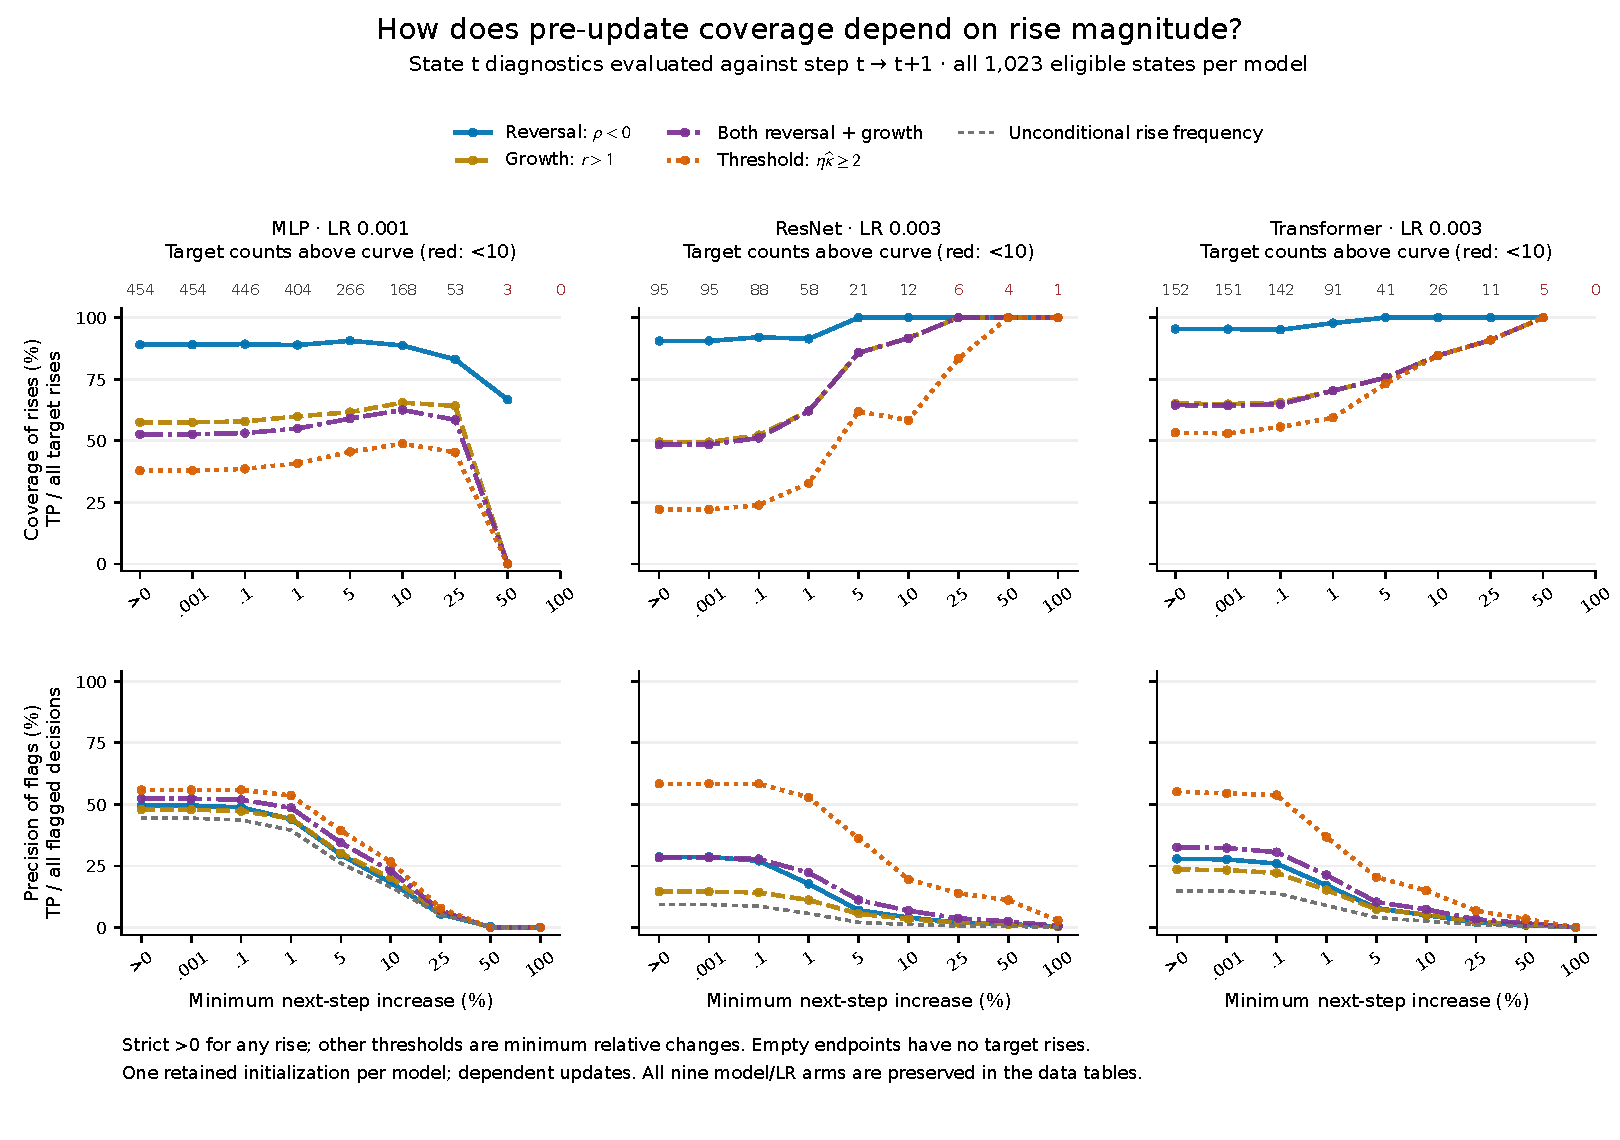
\includegraphics[page=1,width=9.6in]{figures/adam_forward_and_severity.pdf}
\caption{Coverage and precision versus minimum next-step relative loss increase. All 1,023 eligible decisions per model are retained; counts identify rare targets. Reversal, growth, their conjunction, and the projected-response threshold are compared with unconditional frequency.}
\end{figure}
\end{landscape}
\clearpage
\begin{landscape}
\begin{figure}[H]
\centering
\includegraphics[page=2,width=9.6in]{figures/adam_forward_and_severity.pdf}
\caption{Individual loss increases of at least 10 percent at each future offset. All offsets use the same 1,008 decision states. Coverage and precision describe the current flag at that offset; they are not validation of an outcome-selected lead time.}
\end{figure}
\end{landscape}
\clearpage
\begin{landscape}
\begin{figure}[H]
\centering
\includegraphics[page=3,width=9.6in]{figures/adam_forward_and_severity.pdf}
\caption{Net loss increase of at least 10 percent from the decision state to each future horizon. This target differs from an individual future step increase; common decision support is retained.}
\end{figure}
\end{landscape}
\clearpage
\begin{landscape}
\begin{figure}[H]
\centering
\includegraphics[page=4,width=9.6in]{figures/adam_forward_and_severity.pdf}
\caption{Any loss at least 10 percent above the decision-state loss within the future horizon. The target set expands with the horizon, so increasing precision must be compared with its rising base frequency.}
\end{figure}
\end{landscape}
\clearpage
\begin{landscape}
\begin{figure}[H]
\centering
\includegraphics[page=5,width=9.6in]{figures/adam_forward_and_severity.pdf}
\caption{Within-horizon increases restricted to currently non-rising decisions. This excludes an already-rising step but not necessarily an ongoing excursion. Sparse threshold support and target frequencies remain visible.}
\end{figure}
\end{landscape}
\clearpage
\begin{landscape}
\begin{figure}[H]
\centering
\includegraphics[page=6,width=9.6in]{figures/adam_forward_and_severity.pdf}
\caption{Remembered warnings for the unique next-step target. Each target is counted once; all memory widths use decisions 16--1023. Longer memory increases both coverage and the number of non-target flags.}
\end{figure}
\end{landscape}

